\documentclass[svgnames]{standalone}
\usepackage{tikz}
\usetikzlibrary{calc,positioning,backgrounds,arrows}

% Define constants here

\begin{document}
	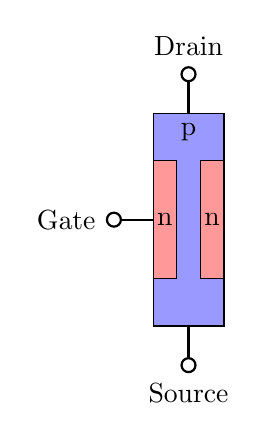
\begin{tikzpicture}[scale=0.3]
			\filldraw[fill=blue!40!white, draw=black] (0,0) -- ++(0,2) -- ++(1,0) -- ++(0,5) -- ++(-1,0) -- ++(0,2) -- ++(3,0) -- ++(0,-2) -- ++(-1,0) -- ++(0,-5) -- ++ (1,0) -- ++(0,-2) -- ++(-3,0)
			;
			\filldraw[fill=red!40!white, draw=black] (0,2) rectangle ++(1,5) node[pos=.5] {n};
			\filldraw[fill=red!40!white, draw=black] (2,2) rectangle ++(1,5) node[pos=.5] {n};
			\draw [thick, -o] (0, 4.5) -- ++(-2,0) node[anchor=east] {Gate};
			\draw [thick, -o] (1.5, 9) -- ++(0,2) node[anchor=south] {Drain};
			\draw (1.5, 9) node[anchor=north] {p};
			\draw [thick, -o] (1.5, 0) -- ++(0,-2) node[-*, anchor=north] {Source};
		\end{tikzpicture}
\end{document}
